% !TEX root = ../thesis-example.tex
%
\section{Light Environment Reproduction}

To conclude by now: We have successfully created an image composition with 
correct projection parameters, recalculated a planar depth, delayed in-engine 
frame times with camera frame timings and realigned the frame rate between both 
image generating systems.

\begin{figure}[htb]
	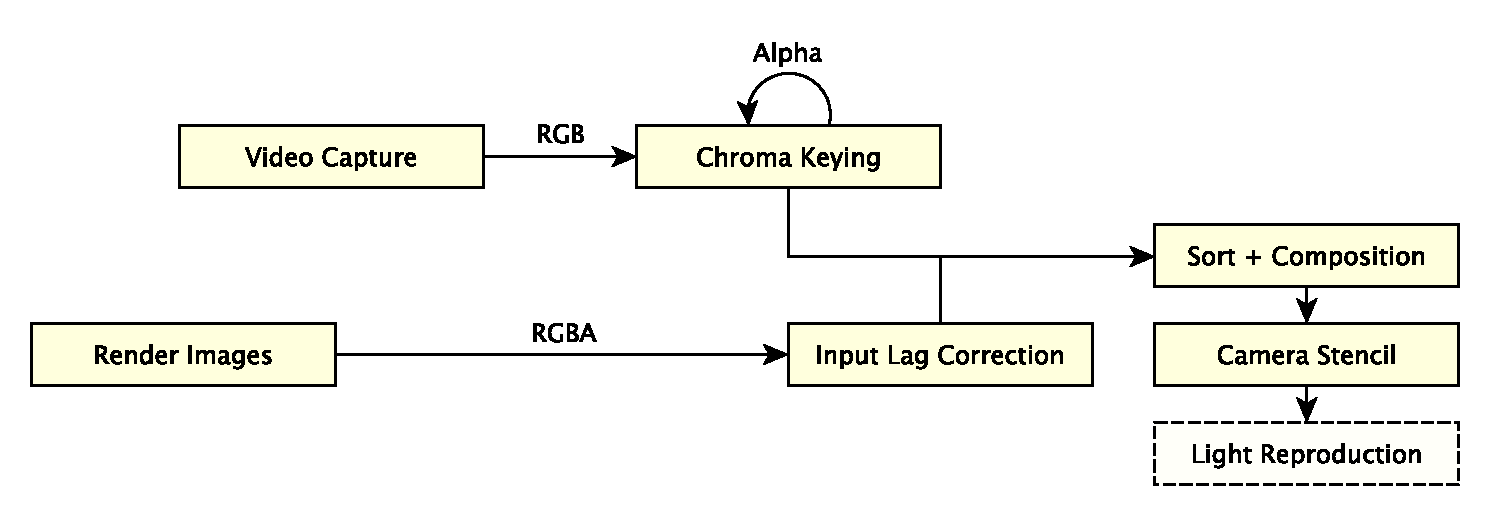
\includegraphics[width=\textwidth]{_raw_resources/pipeline_steps/4_7_lights.pdf}
	\caption{Following in this pipeline is lights reproduction}
	\label{fig:steps:lights}
\end{figure}

A minor last step is light-reproduction, in which an approximate lightning 
setting will be transferred from 3D environment to the video feed of a VR 
actor. Assuming that the video footage contains a natural lit, tint-free and 
calibrated video signal, it is possible to approximate how a VR actor would 
be lit like if he truly was inside a virtual environment.

\begin{figure}[htb]
	\includegraphics[width=\textwidth]{_raw_resources/light-reconstruction/comparison.jpg}
	\caption{Left: original, Right: reconstruction}
	\label{fig:light-reconstruction:comparison}
\end{figure}

\begin{figure}[htb]
	\includegraphics[width=\textwidth]{_raw_resources/light-reconstruction/color_difference.png}
	\caption{Color difference by substracting a reconstruction from the 
	original.}
	\label{fig:light-reconstruction:difference}
\end{figure}

\begin{figure}[htbp]
	\caption{A comparison of different composition methods in engine}
	\label{fig:light-reconstruction:diff-capture}
	\begin{subfigure}[t]{.45\textwidth}
		\centering
		\includegraphics[width=\textwidth]{_raw_resources/light-reconstruction/capture.png}
		\caption{captured, lit plane}
	\end{subfigure}
	\begin{subfigure}[t]{.45\textwidth}
		\centering
		\includegraphics[width=\textwidth]{_raw_resources/light-reconstruction/color_difference.png}
		\caption{Color difference by substracting a reconstruction from the 
			original.}
	\end{subfigure}
\end{figure}

Ambient light reproduction hinges on two assumptions: An actors recorded video 
is flat for this purpose and he receives a clean and consistent light from all 
angles that has no additional glossiness. With that we can have project a plane 
at the actors position, filling the frustum edges of another virtual camera 
with the same camera projection parameters from section 
\ref{sec:projection-params}. This plane contains a simple lit material with 
white albedo coloring, which captures the lightning situation at this given 
point (figure \ref{fig:light-reconstruction:diff-capture} a).

To calculate the position $P_{pos}$ and size $\vec{P_{x, y}}$ with a 
given forward vector $\vec{C_{forward}}$ and position $C_{pos}$ of the 
camera, as well as a distance $Z$ between camera and actor and a current Field 
of View $FoV$ in radians by assuming a 16:9 video feed:

\eq{eq:light-reproduction:pos}{
	P_{pos} = C_{pos} + Z * \vec{C_{forward}}
}

\eq{eq:light-reproduction:size:1}{
	P_{x, y} =
	\begin{bmatrix}
		2 * \tan(FoV / 2) * Z \\
		P_{x} * \frac{16}{9}
	\end{bmatrix}	
}